% see A1.4
\chapter{Planen}
\label{ch:plan}

Die Zeitplanung wird in der Abbildung \ref{fig:timeplan} oberhalb gezeigt. Die restlichen Aspekte der Planung sind in diesem Kapitel dokumentiert.

\section{Anwendungsfälle}

\newpage

\section{Datenmodell}

\subsection{Entity-relationship Diagramm}

Das Entity-relationship Diagramm \ref{fig:erd} zeigt alle für diese PA notwendigen Entitäten und deren Verhältnis zueinander. Die Felder
der einzelnen Tabellen können in der Planungsphase noch nicht vollumfänglich definiert werden und werden höchstwahrscheinlich in einzelnen Fällen während der Realisierungsphase
erweitert. Das Grundkonzept und die Assoziationen zwischen den verschiedenen Entitäten bleiben allerdings gleich.

Die drei Entitäten \emph{active\_storage\_attachment}, \emph{active\_storage\_blob} und \emph{action\_text\_rich\_text} werden automatisch durch das
Framework generiert und sollen in diesem Diagramm zum besseren Verständnis des Gesamtkonzeptes beitragen. In der Praxis wird man mit diesen Tabellen direkt kaum etwas zu tun haben.
Diese werden von den zwei gems ActiveStorage und ActionText verwendet, welche das Einbinden von formatierten Textinhalten und Dateiuploads ermöglichen.

\begin{figure}[H]
    \centering
    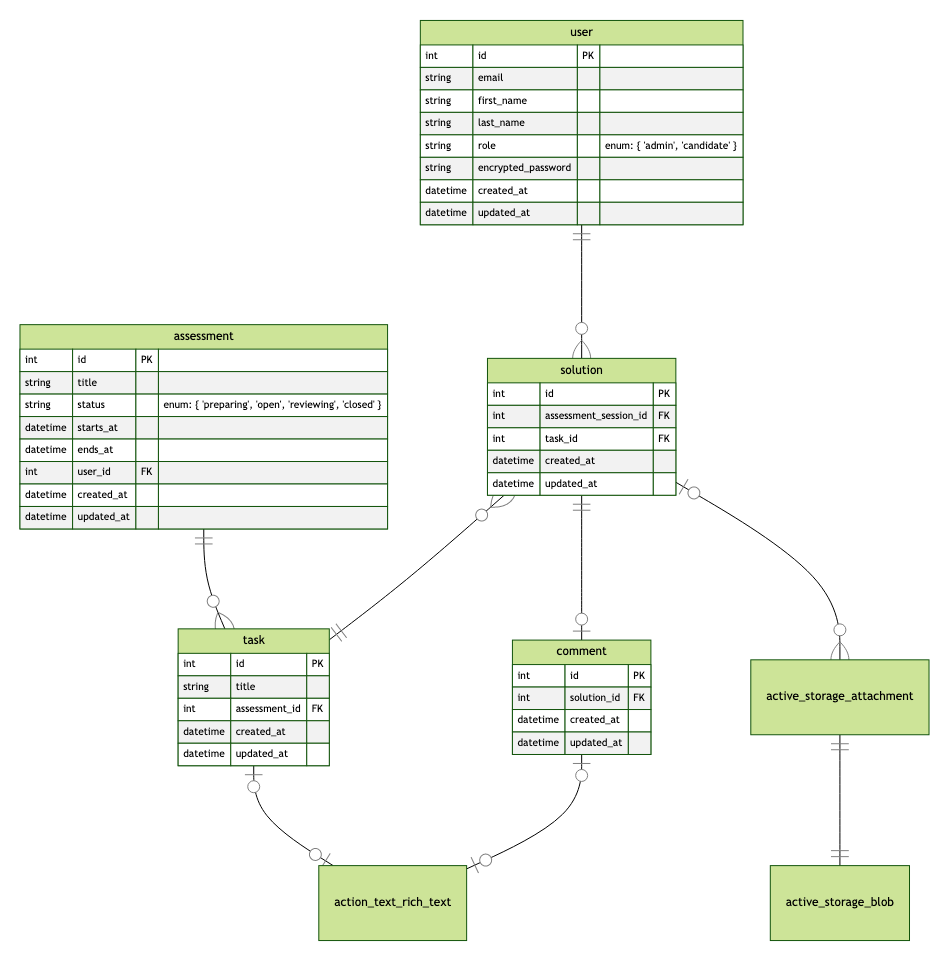
\includegraphics[height=15cm]{images/diagrams/entity-relation.png}
    \caption{\label{fig:erd} Entity-relationship Diagramm}
\end{figure}

\newpage

Sowohl der Zustand (State) von einem \emph{assessment} als auch die Benutzerrolle von einem \emph{user} wird in Form eines Enums abgebildet. Dabei ist zu beachten, dass es in der Praxis kein Database-Level Enum sein wird,
sondern der Wert in Form eines Strings in der Datenbank gespeichert werden soll. Der Constraint wird dann auf Application-Level durchgesetzt. Das ist ein ActiveRecord Standard und ermöglicht eine höhere Flexibilität und Erweiterbarkeit.
Ausserdem werden nicht alle Akteure aus \ref{tab:participants} in Form von Benutzerrollen in der \emph{user} Entität abgebildet, da die Zwei Akteure \enquote{Betreuer} und \enquote{Korrektor} in der Praxis die gleiche Person sein wird.

\subsection{Physisches Datenmodell (Generation)}

Das Ruby on Rails Framework bietet verschiedenste Command-Line Utilities, mit denen man sich relativ einfach gewisse
Grundstrukturen automatisiert generieren lassen Kann. Abgeleitet von \ref{fig:erd} können nun die ganzen Commands aufgestellt werden.
Werden diese ausgeführt, erstellen diese sowohl die dazugehörigen Model-Klassen, als auch alle notwendigen Datenbankmigrationen.

Die ganzen Assoziationen zwischen den Entitäten werden mit dem \emph{references} Typ schon bei der Generation abgebildet.
Bei dem \emph{rich\_text} Feldtyp handelt es sich um die bereits angesprochenen formatierten Textinhalte,
welche automatisch in eine andere Tabelle ausgelagert werden. Bei einem \emph{attachment} handelt es sich um einen anhängenden File-Upload.

\begin{figure}[H]
\begin{codebox}[]
\begin{minted}{shell}
bin/rails generate model Task title:string body:rich_text assessment:references
bin/rails generate model Assessment title:string status:string starts_at:datetime ends_at:datetime
bin/rails generate model Solution files:attachments task:references task:references user:references
bin/rails generate model Comment body:rich_text solution:references 
\end{minted}
\end{codebox}
\caption{\label{fig:generate-models}Commands für die automatisierte Generation von Model-Klassen}
\end{figure}

\newpage

\section{Zustandsdiagramm}

Während dem Lebenszyklus von einem \emph{assessment} durchläuft dieses mehrere Zustände. Diese ändern
sich durch Interaktionen gewisser Akteure mit dem System. Der Zustand verläuft relativ linear von einem Zustand zum nächsten und es gibt keine Abzweigungen
oder sonstige Sonderfälle. Das Diagramm \ref{fig:state-diagram} versucht diesen Prozess zu veranschaulichen.

Zwischen den Zuständen gibt es jeweils einen \emph{Trigger}, eine \emph{[Guard]} oder einen \emph{/Effect}.

\begin{figure}[H]
    \centering
    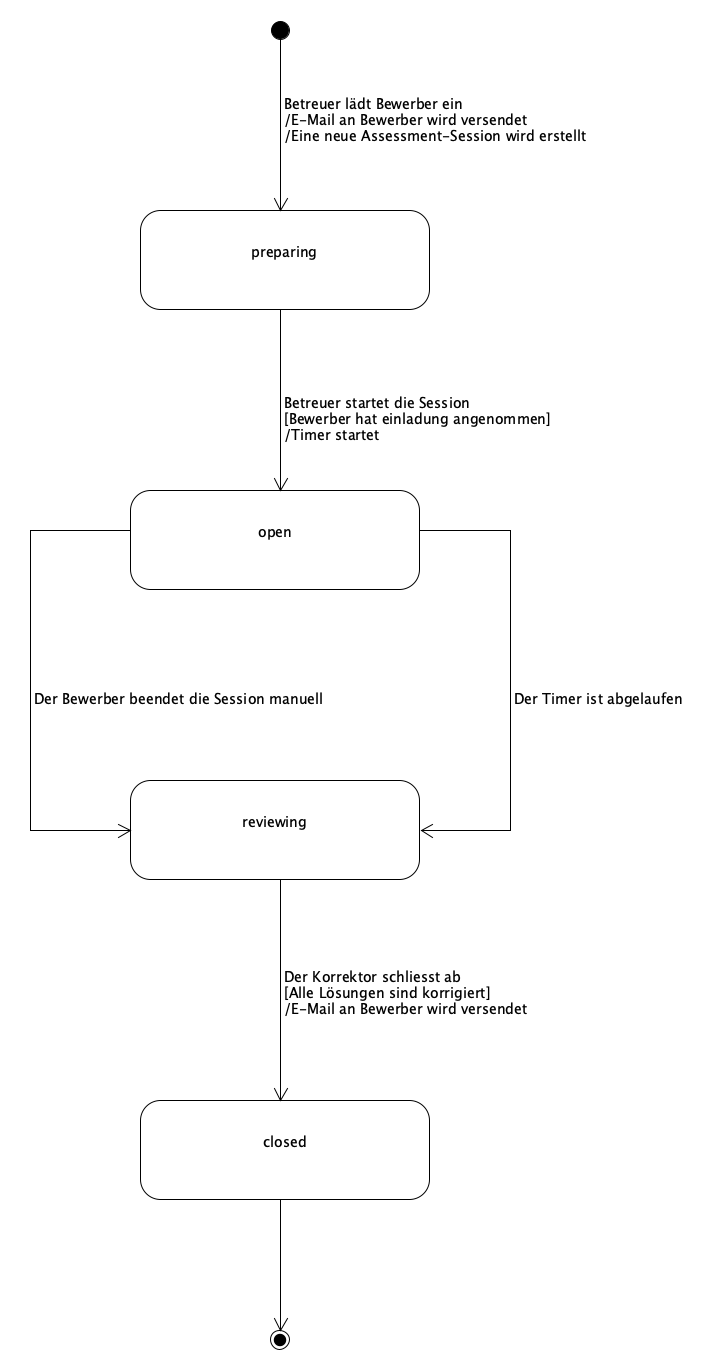
\includegraphics[height=17cm]{images/diagrams/state.png}
    \caption{\label{fig:state-diagram}UML Zustandsdiagramm eines Assessments}
\end{figure}

\newpage

\section{Mockups}

In diesem Abschnitt folgen grobe Entwürfe der verschiedenen Ansichten der Applikation. Diese sollen die Realisierung
erheblich vereinfachen und verschaffen nicht nur einen Überblick über das UI-Design, sondern auch über die genaueren
Funktionalitäten und Benutzer-Flows der Applikation. Die Entwürfe wurden ausserdem nach den Akteuren \ref{tab:participants} kategorisiert.

Beim Design wurde darauf geachtet, es möglichst minimalistisch zu halten und strikt der Aufgabenstellung zu folgen. Es wurden keine überflüssigen Elemente
eingebaut um sowohl die Realisierung als auch die spätere Nutzung der Applikation zu vereinfachen.

Ausserdem wurde das UI in englisch gestaltet, da es die Firmensprache in der Renuo AG ist.

\subsection{Bewerber}
\begin{figure}[H]
    \centering
    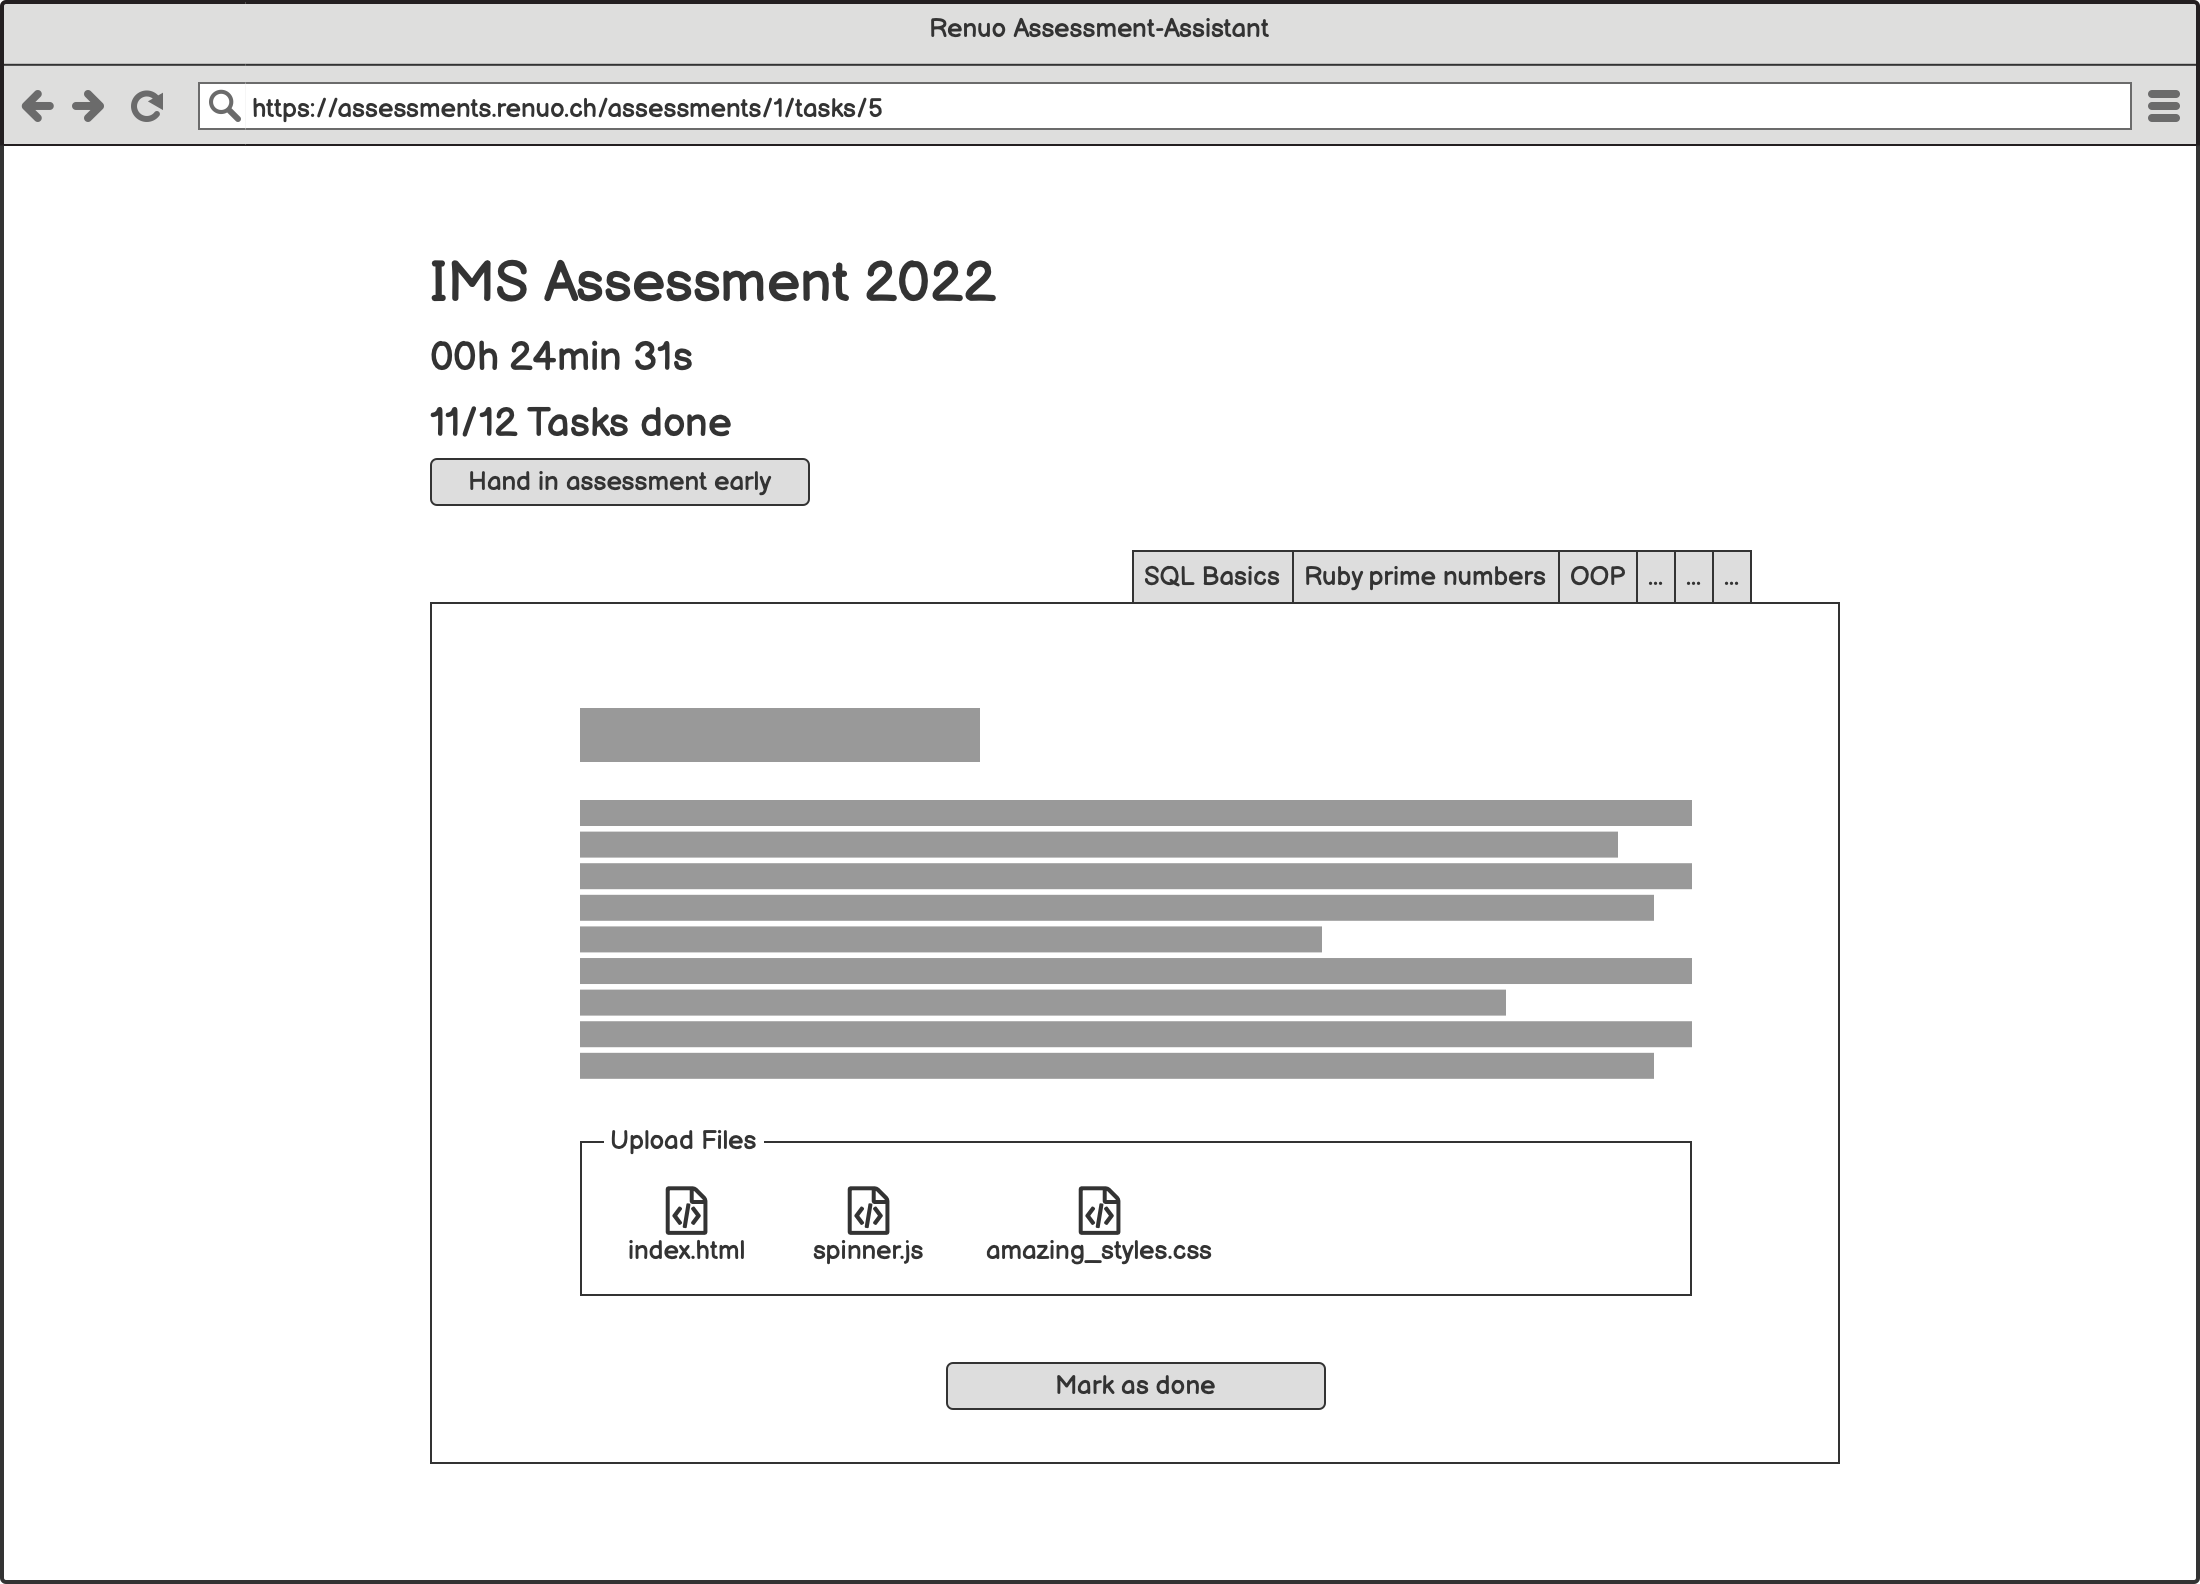
\includegraphics[width=12cm]{images/mockups/candidate-solve-assessment.png}

    \caption{\label{fig:mockup-candidate-solve-assessment}Entwurf für das Lösen eines Assessments}
\end{figure}

\subsection{Betreuer}
\begin{figure}[H]
    \centering
    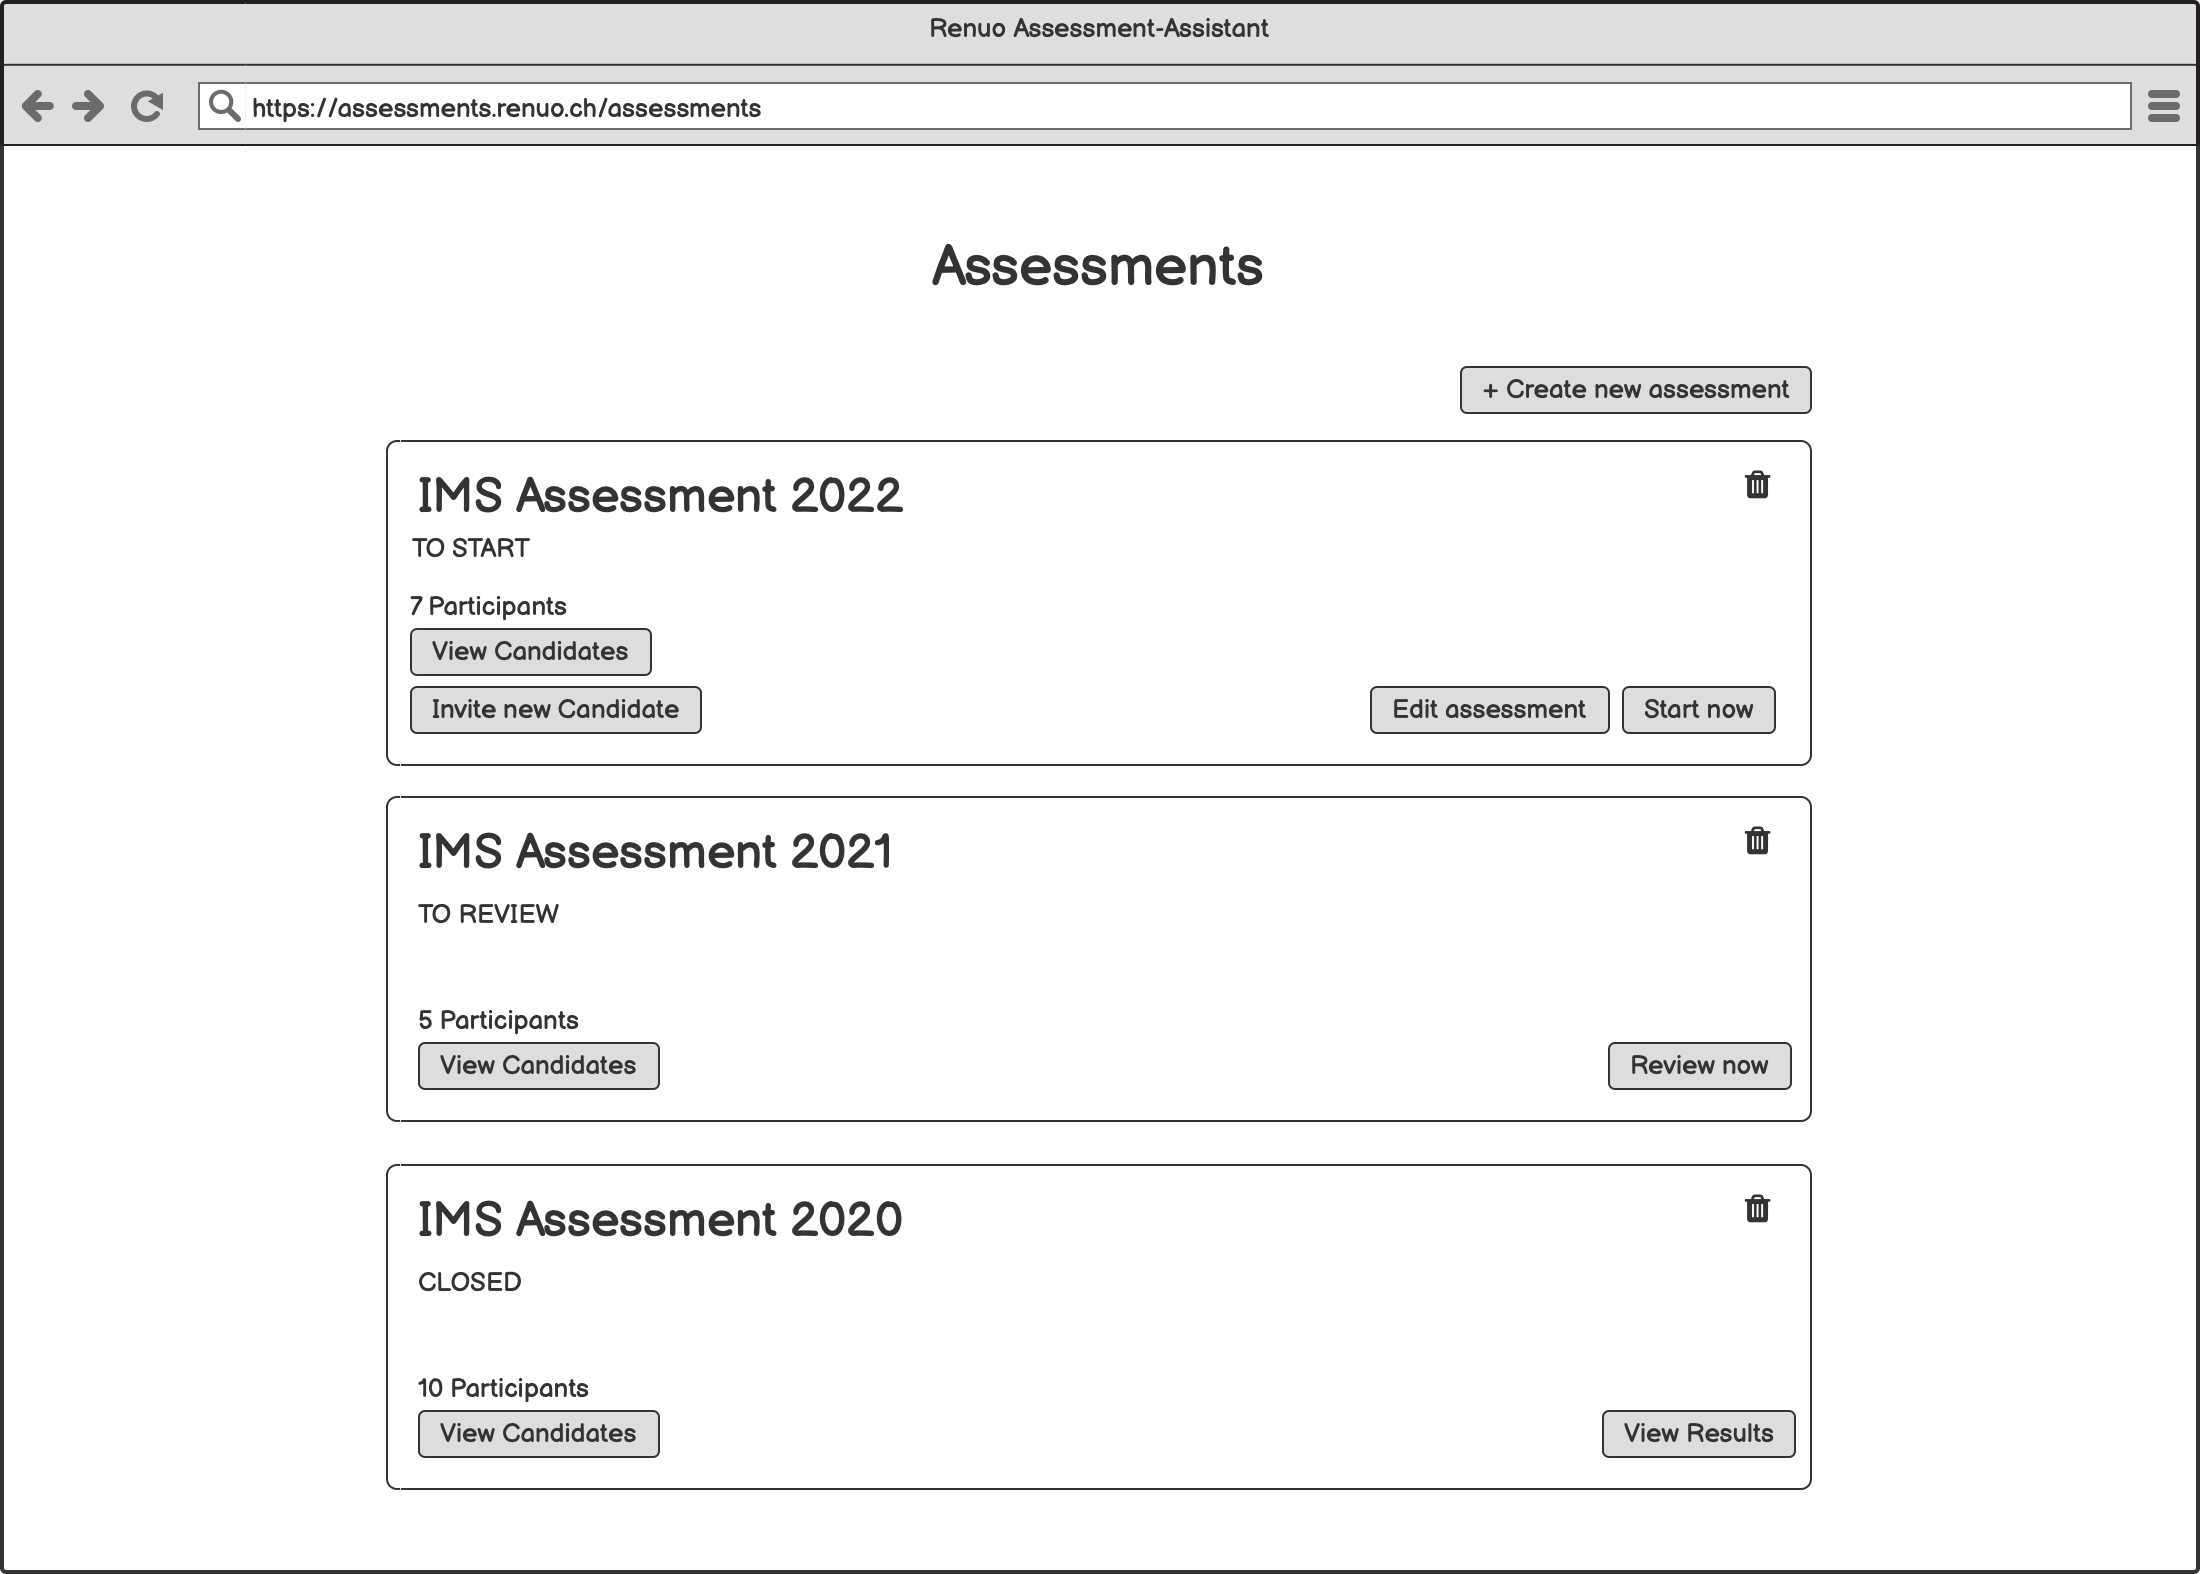
\includegraphics[width=12cm]{images/mockups/supervisor-list-assessments.png}
    \caption{\label{fig:mockup-supervisor-list-assessments}Entwurf für das Auflisten von Assessments}
\end{figure}
\begin{figure}[H]
    \centering
    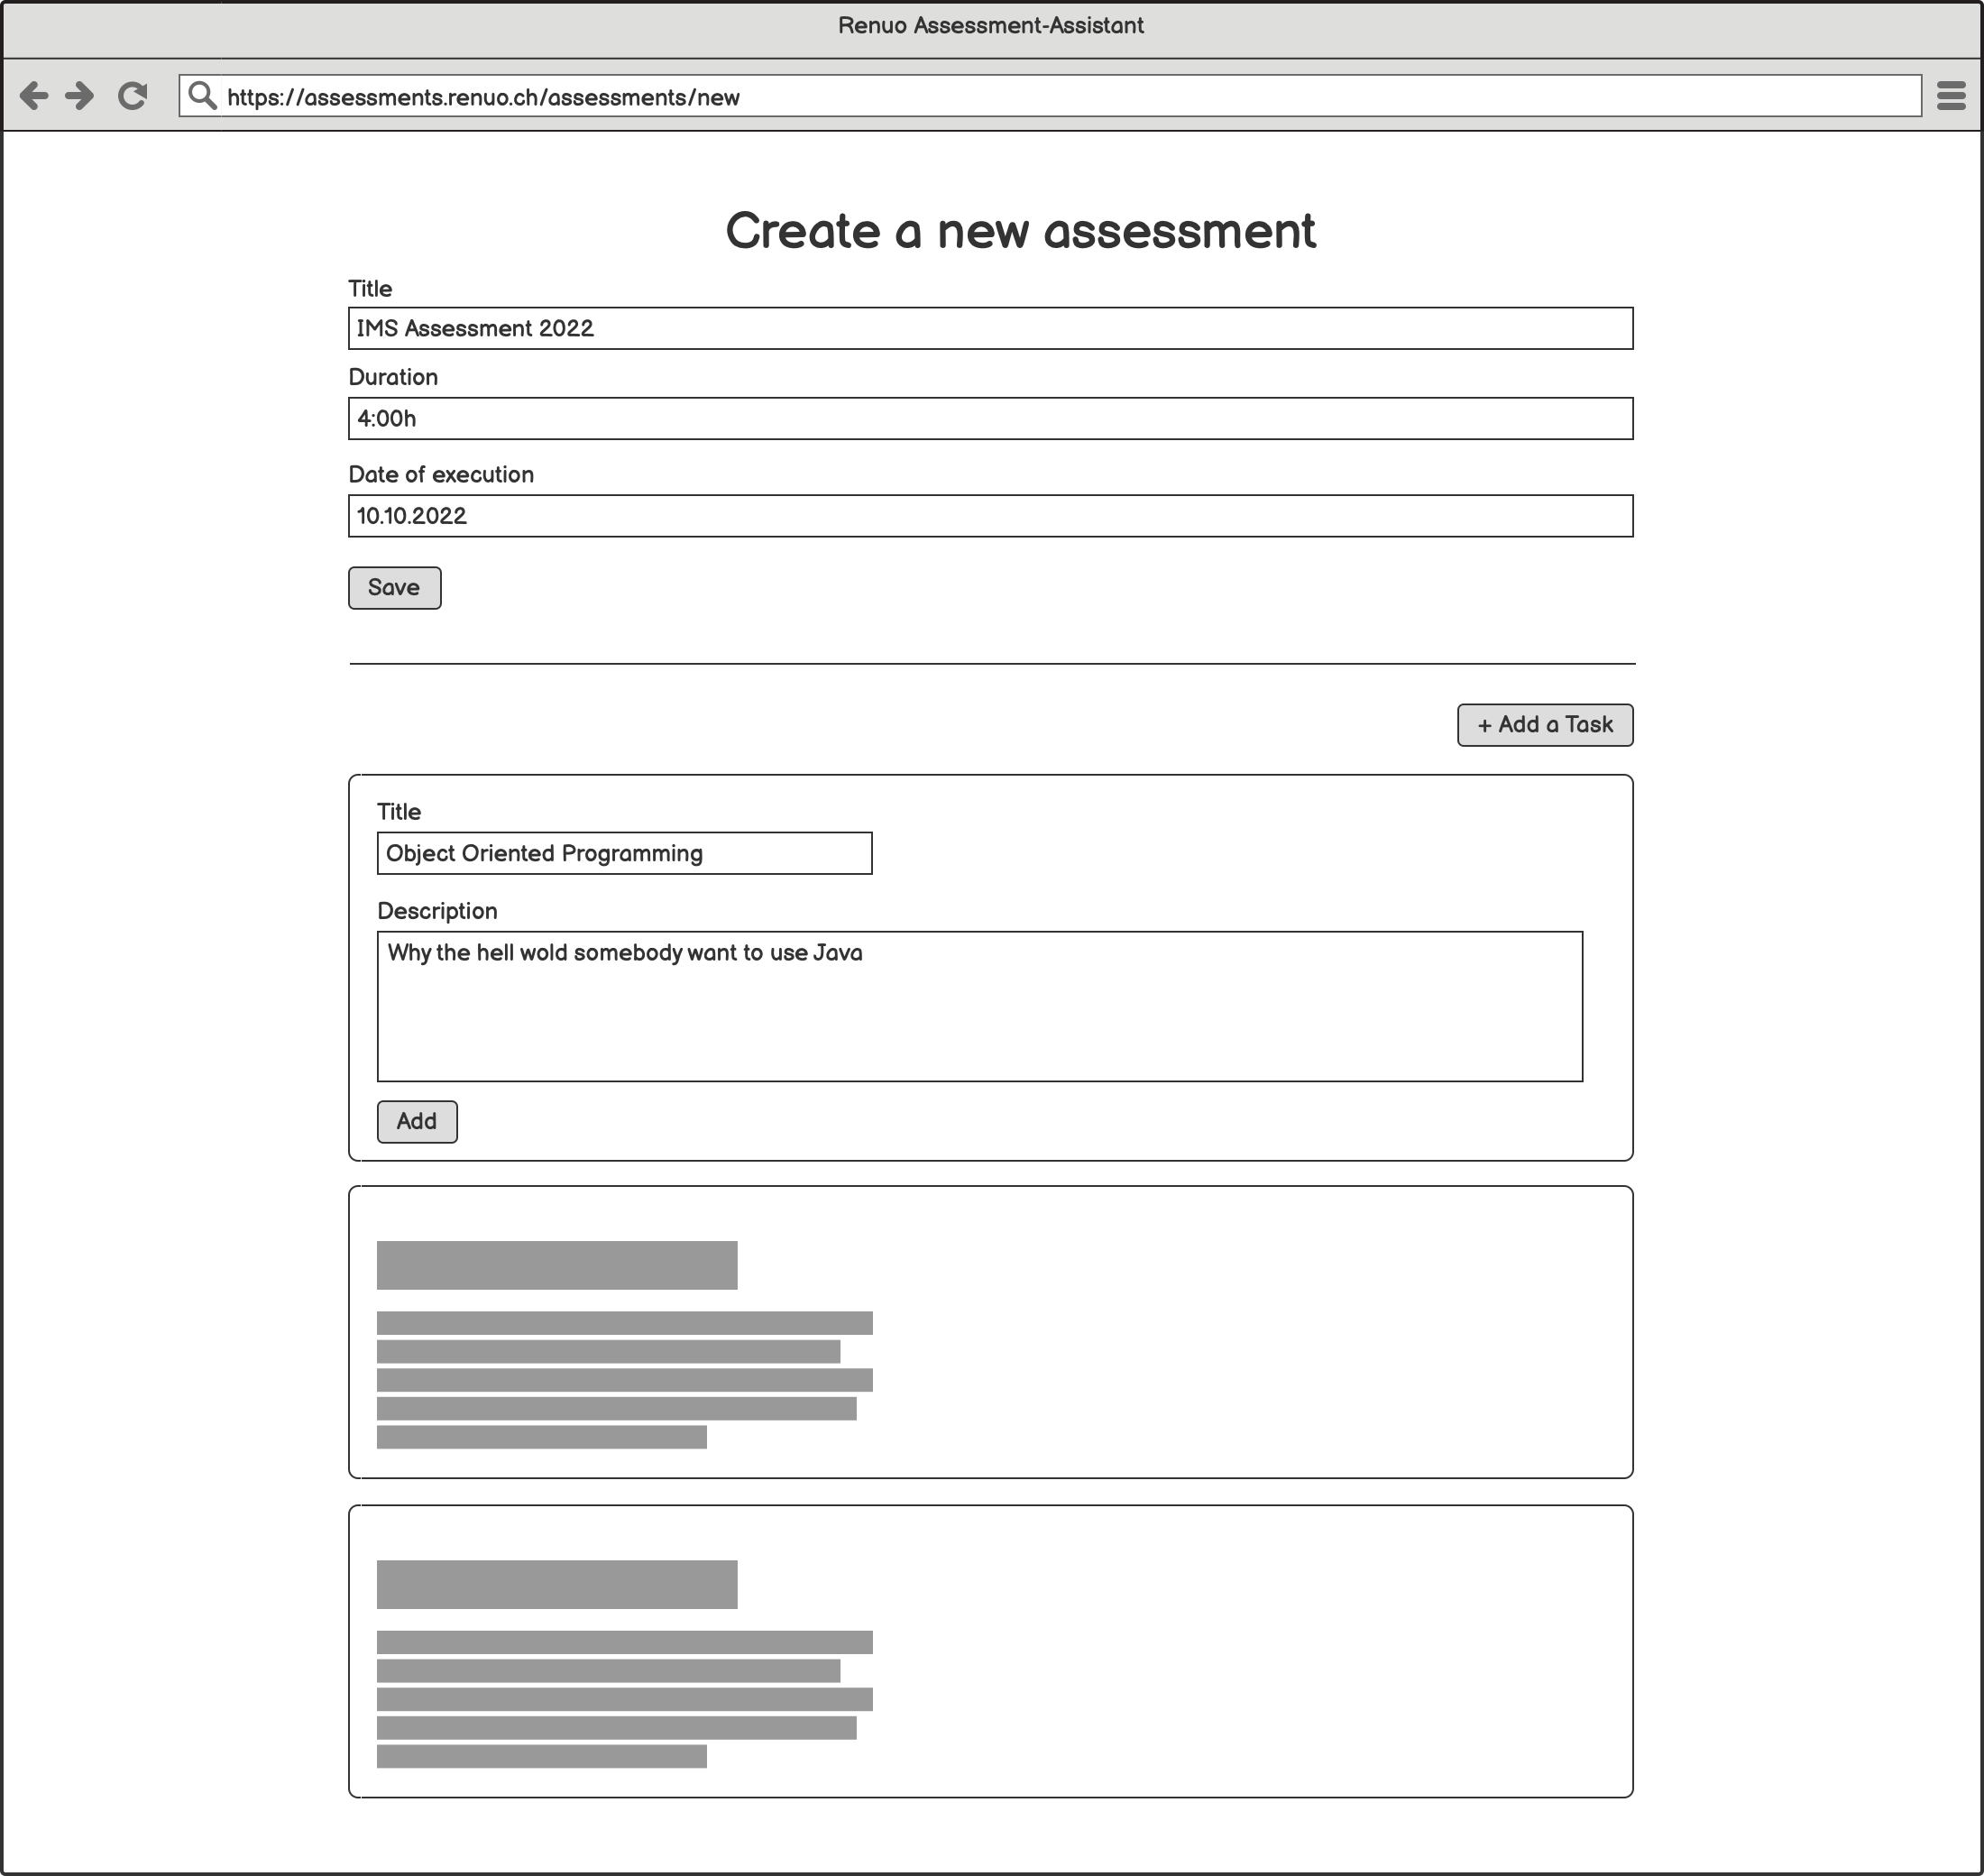
\includegraphics[width=12cm]{images/mockups/supervisor-create-assessment.png}
    \caption{\label{fig:mockup-supervisor-create-assessment}Entwurf für das Erstellen eines neuen Assessments}
\end{figure}

\subsection{Korrektor}
\begin{figure}[H]
    \centering
    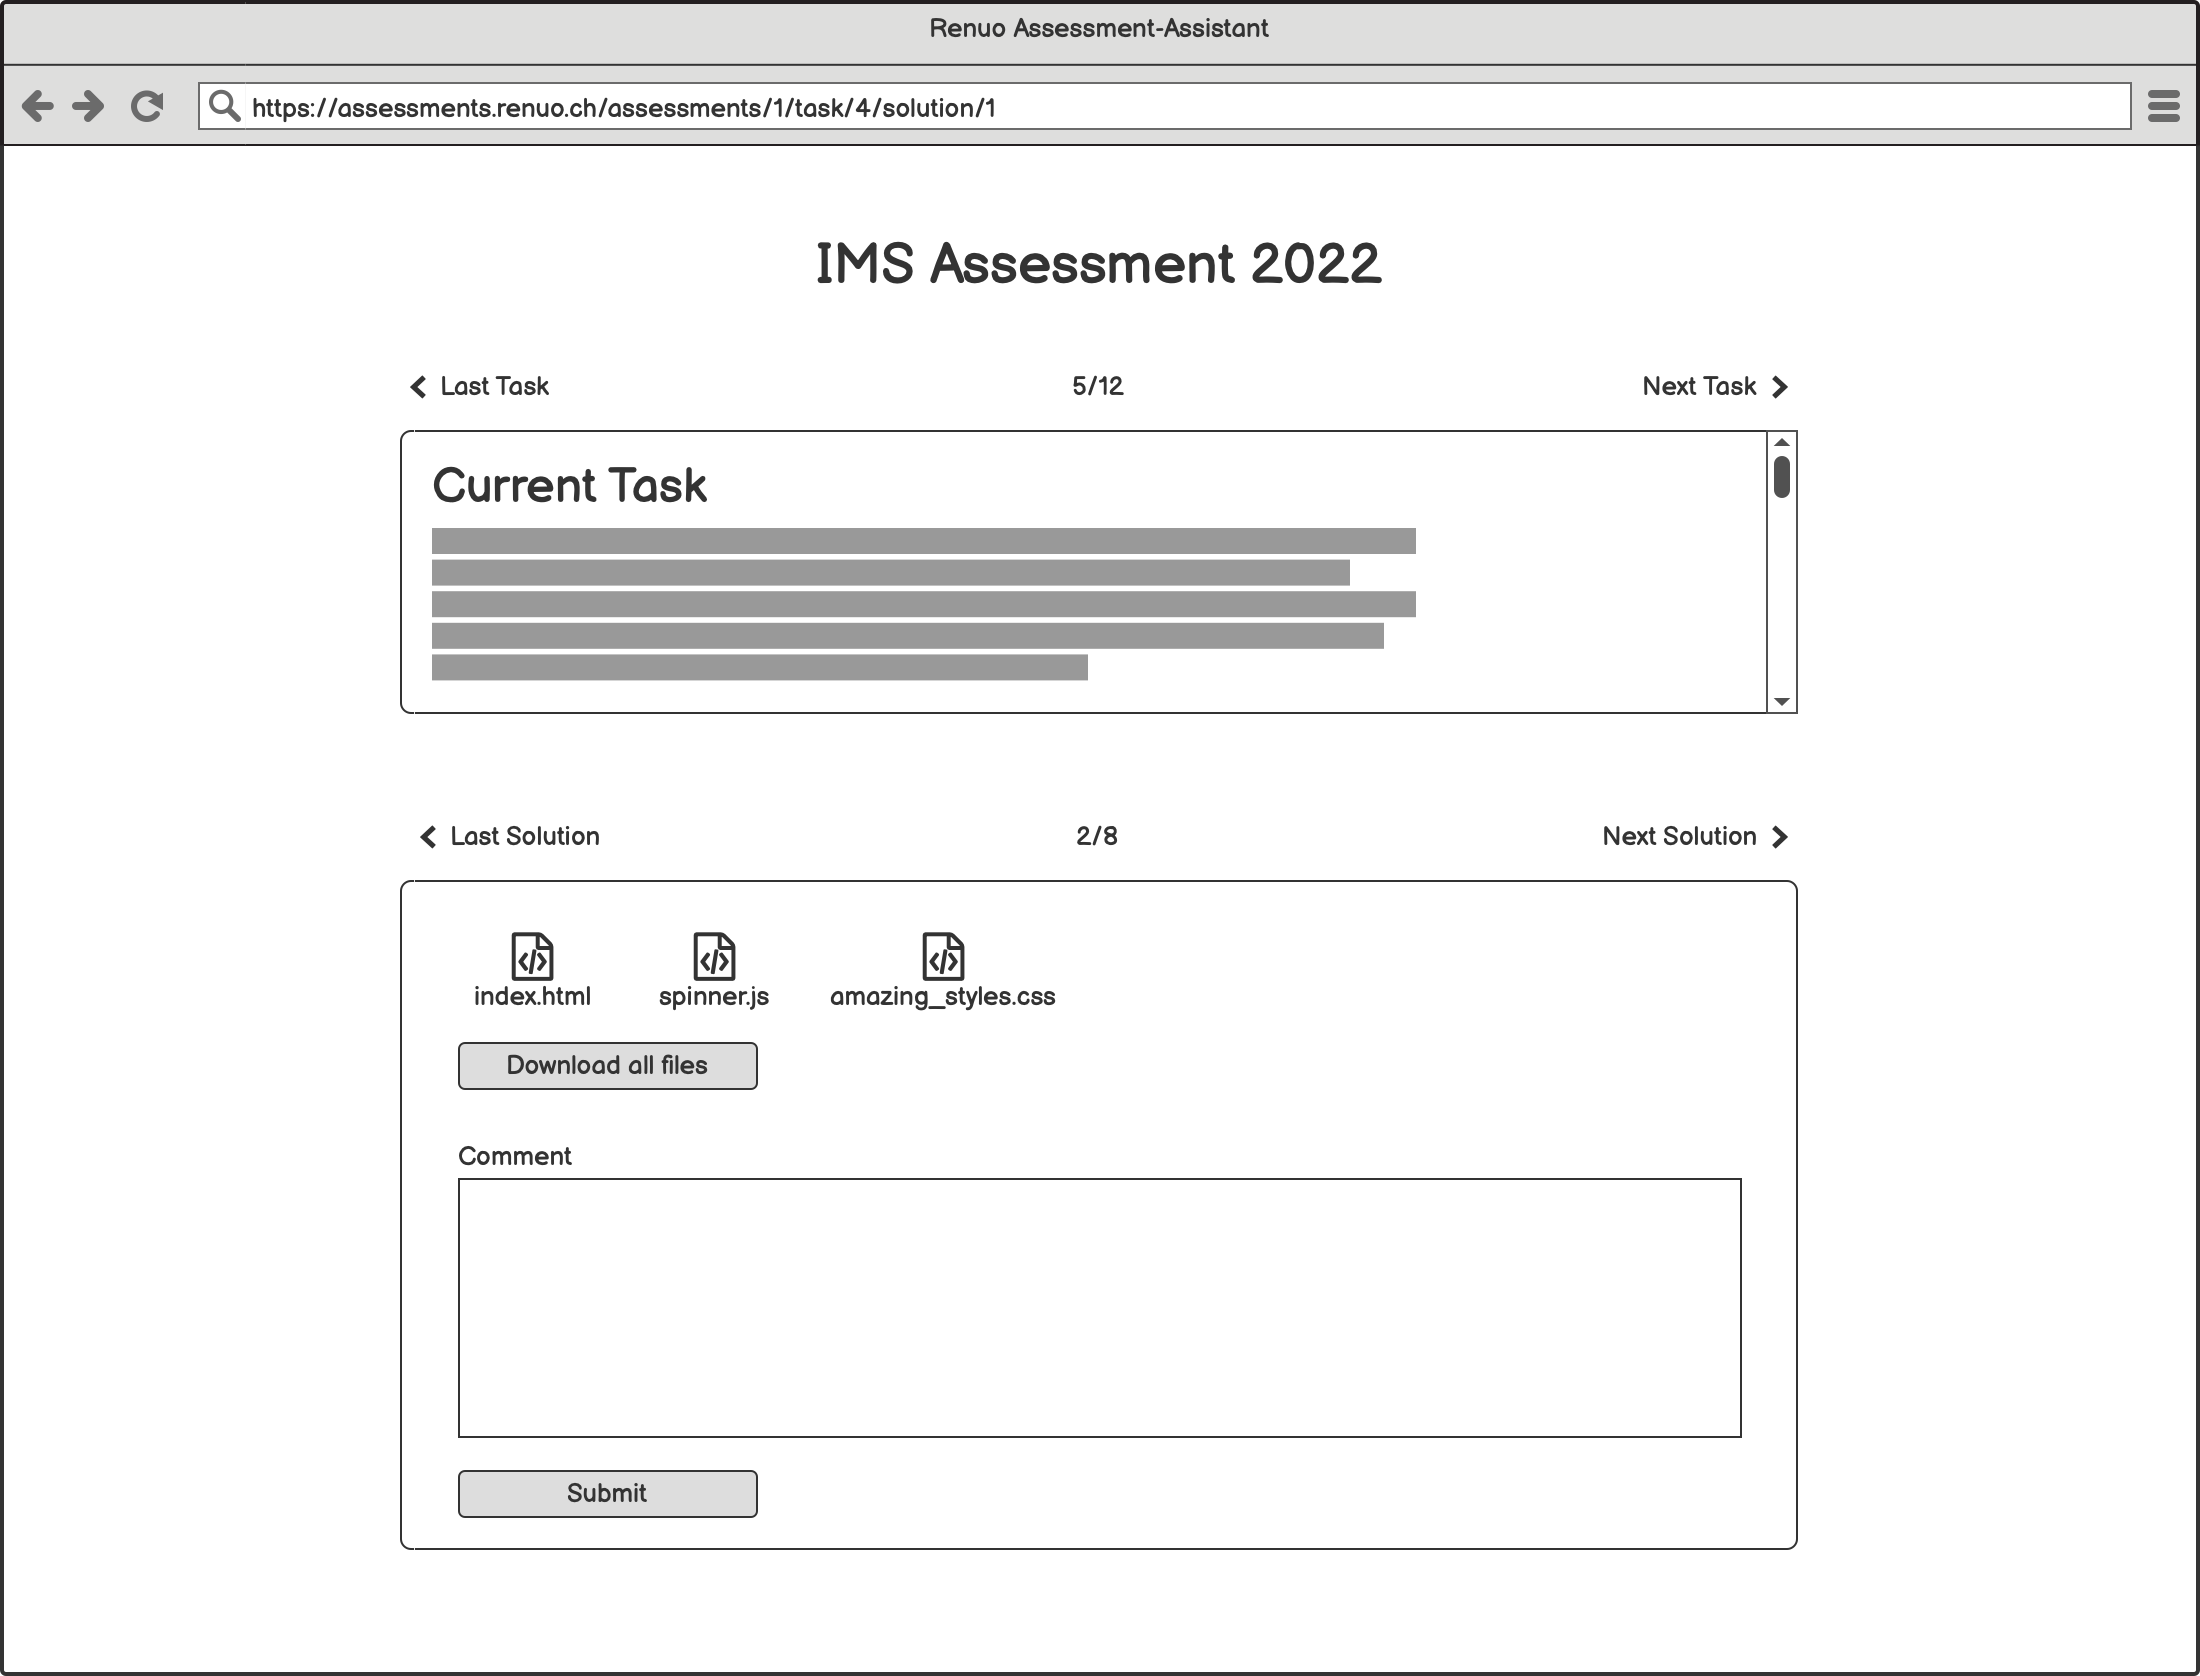
\includegraphics[width=12cm]{images/mockups/corrector-correct-assessment.png}
    \caption{\label{fig:mockup-solve-assessment}Entwurf für das Korrigieren eines Assessments}
\end{figure}
\begin{figure}[H]
    \centering
    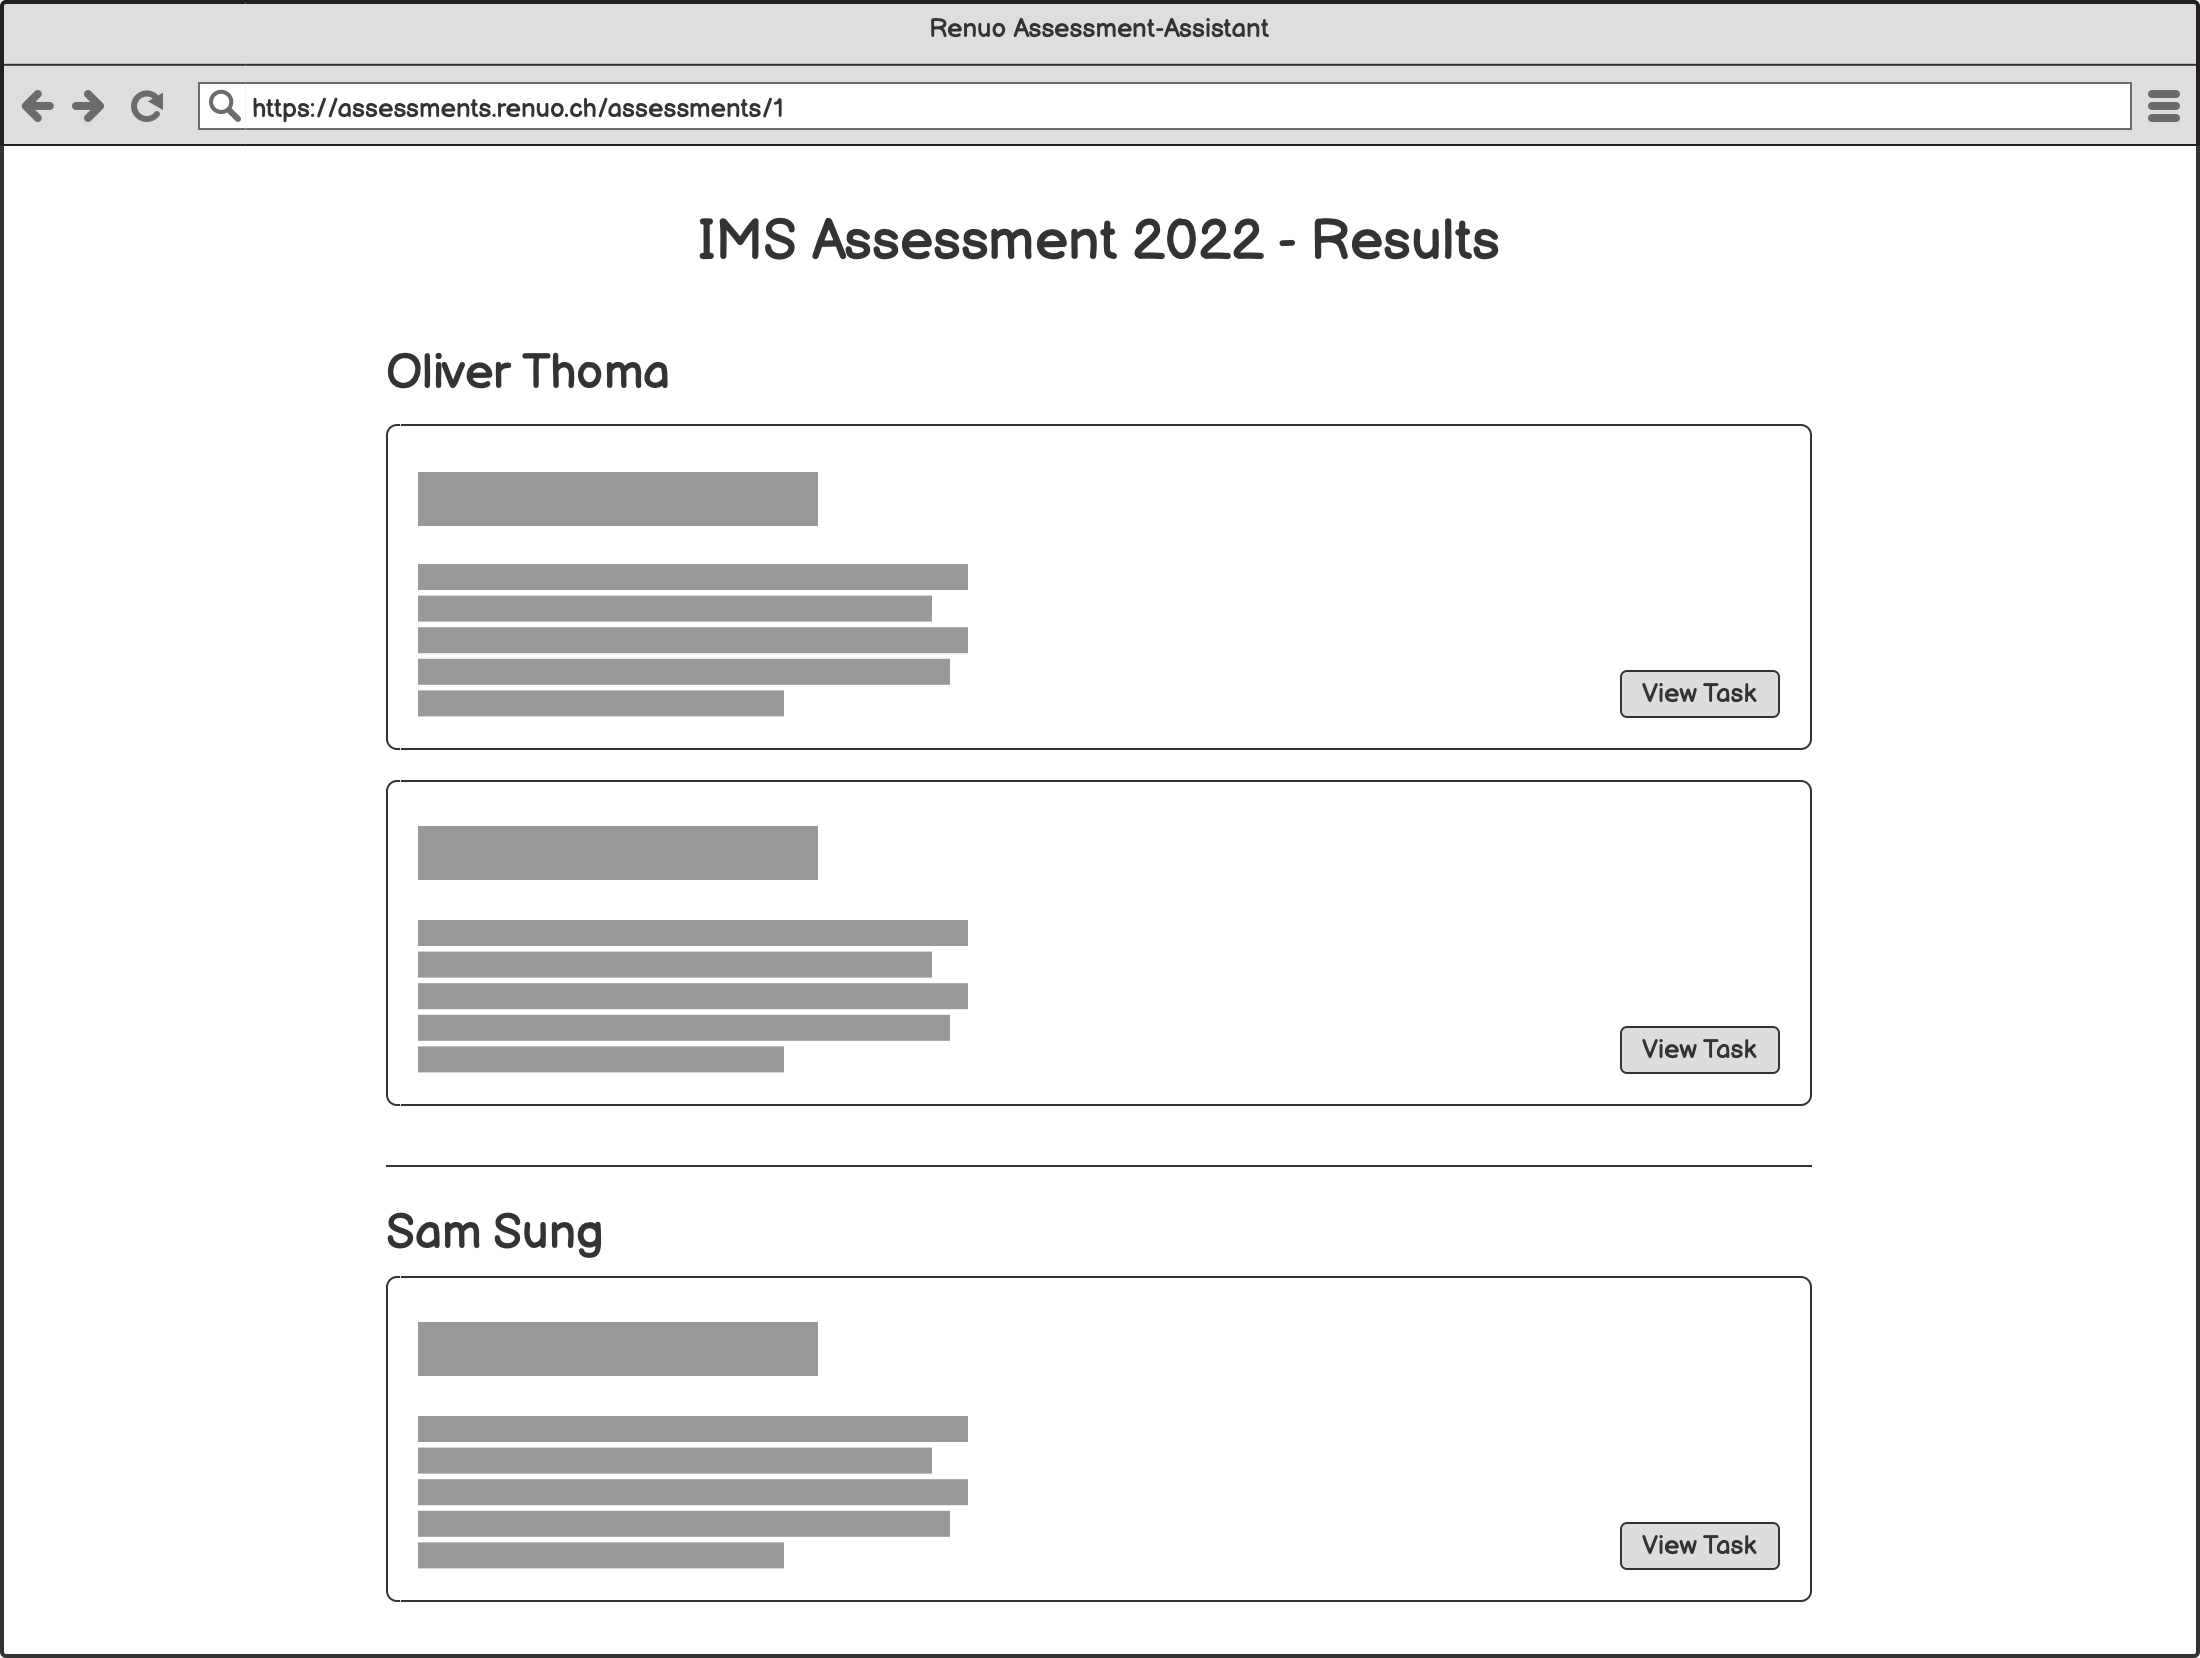
\includegraphics[width=12cm]{images/mockups/assessment-results.png}
    \caption{\label{fig:mockup-assessment-results}Entwurf für das Einsehen und Auflisten der Korrekturen}
\end{figure}

\newpage

\section{Testkonzept}

Das Testkonzept beschreibt, wie und mit welchen Werkzeugen das Resultat auf seine Richtigkeit kontrolliert wird.

\subsection{Automatisierte Tests}

Grundsätzlich wird versucht eine Testabdeckung von 100\% durch automatisierte Tests zu erreichen. Die einzelnen
Ziele/Meilensteine der Realisierungsphase werden in dieser PA testgetrieben implementiert. Das heisst, es werden zu Beginn
Unit- und Integrationtests geschrieben und erst dann wird die eigentliche Funktionalität implementiert, bis alle Tests bestehen. Dies ermöglicht
ein effizientes arbeiten, da über die exakte Implementation bereits im Vorraus nachgedacht wurde und es garantiert immer eine vollständige Testabdeckung.

Als Testmittel werden folgende Softwarebibliotheken eingesetzt:
\begin{itemize}
    \item RSpec
    \item Capybara
    \item FactoryBot
    \item Faker
\end{itemize}

Das Framework benutzt standardmässig eine dedizierte Testdatenbank, die nach jedem Test gereinigt wird. So gibt es keine Abhängigkeiten
oder Konflikte unter einzelnen automatisierten Tests. Die zwei gems \emph{FactoryBot} und \emph{Faker} ermöglichen ausserdem möglichst
Realitsätsnahe und Konstistente Testdaten- und Strukturen.

\subsubsection{Unit Tests}
Alle Model-, Helper- und Service-Klassen werden mittels RSpec Unit-Tests getestet. Diese sollen überprüfen,
ob die einzelnen Komponenten so Arbeiten, wie diese es beabsichtigen.

\subsubsection{Integration Tests}
Die Controller werden per RSpec Integration-Test getestet. So werden alle Komponenten im Stack der Applikation von ganz oben
nach ganz unten getestet und es wird eine korrekte Integration der darunterliegenden Komponenten sichergestellt.

\subsubsection{System Tests}
Für die einzelnen Flows aller Akteure werden System Tests mit Capybara geschrieben.
Diese öffnen einen headless Chromium Browser und klicken sich automatisiert durch eine im Vorraus definierte Sequenz durch.

\newpage

\subsection{Manuelle Tests}

Die automatisierten Tests decken bereits den grössten Teil der Applikation ab, jedoch gibt es dennoch Teile, die nur im Kontext
des Gesamtsystems getestet werden können. Die folgenden manuellen Tests sollen demnach die vollständige Funktionalität und Integration in die Produktions-Umgebung sicherstellen.

\begin{tabularx}{\textwidth}[H]{|c|X|}
    \hline
    ID & 
    \lipsum[1][1]
    \\ \hline
    
    Beschreibung & 
    \lipsum[1][1]
    \\ \hline

    Vorraussetzung & 
    \lipsum[1][1]
    \\ \hline

    Schritte & \lipsum[1][1]
    \\ \hline

    Erwartetes Ergebnis & 
    \lipsum[1][1]
    \\ \hline
\end{tabularx}

\begin{tabularx}{\textwidth}[H]{|c|X|}
    \hline
    ID & 
    \lipsum[1][1]
    \\ \hline
    
    Beschreibung & 
    \lipsum[1][1]
    \\ \hline

    Vorraussetzung & 
    \lipsum[1][1]
    \\ \hline

    Schritte & \lipsum[1][1]
    \\ \hline

    Erwartetes Ergebnis & 
    \lipsum[1][1]
    \\ \hline
\end{tabularx}

\begin{tabularx}{\textwidth}[H]{|c|X|}
    \hline
    ID & 
    \lipsum[1][1]
    \\ \hline
    
    Beschreibung & 
    \lipsum[1][1]
    \\ \hline

    Vorraussetzung & 
    \lipsum[1][1]
    \\ \hline

    Schritte & \lipsum[1][1]
    \\ \hline

    Erwartetes Ergebnis & 
    \lipsum[1][1]
    \\ \hline
\end{tabularx}

\begin{tabularx}{\textwidth}[H]{|c|X|}
    \hline
    ID & 
    \lipsum[1][1]
    \\ \hline
    
    Beschreibung & 
    \lipsum[1][1]
    \\ \hline

    Vorraussetzung & 
    \lipsum[1][1]
    \\ \hline

    Schritte & \lipsum[1][1]
    \\ \hline

    Erwartetes Ergebnis & 
    \lipsum[1][1]
    \\ \hline
\end{tabularx}

\begin{tabularx}{\textwidth}[H]{|c|X|}
    \hline
    ID & 
    \lipsum[1][1]
    \\ \hline
    
    Beschreibung & 
    \lipsum[1][1]
    \\ \hline

    Vorraussetzung & 
    \lipsum[1][1]
    \\ \hline

    Schritte & \lipsum[1][1]
    \\ \hline

    Erwartetes Ergebnis & 
    \lipsum[1][1]
    \\ \hline
\end{tabularx}
